\documentclass[a4paper]{article}
\usepackage{amsmath}
\usepackage{graphicx}
\usepackage[bookmarks=true]{hyperref}
\usepackage[left=2cm, right=2cm]{geometry}



\title{Politecnico di Milano\\
Formal Methods for Concurrent \\
and \\
Real-time Systems\\
Homework project\\
\textbf{Collaborative Robotics Modeling }}
\author{Aldeghi Gabriele \\
  Mantovani Mirko \and
  Sacco Alessio \\
  Sonzogni Stefano}
 \date{\today}
 



% The other logical operators are: \lnot, \land, \lor, \iff
\newcommand{\liff}{\iff}
\DeclareMathOperator{\limply}{\Rightarrow}
\DeclareMathOperator{\future}{Future}
\DeclareMathOperator{\past}{Past}
\DeclareMathOperator{\lastsOp}{Lasts}
\newcommand{\lasts}{\lastsOp_{ee}}
\DeclareMathOperator{\lastedOp}{Lasted}
\newcommand{\lasted}{\lastedOp_{ei}}
\DeclareMathOperator{\always}{Always}
\DeclareMathOperator{\sometimeFuture}{SometimeFut}
\DeclareMathOperator{\sometimePast}{SometimePast}
\DeclareMathOperator{\withinOp}{Within}
\newcommand{\within}{\withinOp_{ee}}
\DeclareMathOperator{\uptonow}{UpToNow}
\DeclareMathOperator{\becomes}{Becomes}
\DeclareMathOperator{\nexttime}{NextTime}
\DeclareMathOperator{\lasttime}{LastTime}
\DeclareMathOperator{\until}{Until}
\DeclareMathOperator{\since}{Since}


\begin{document}
\maketitle
\begin{center}
	
\includegraphics[width=7cm]{images/polimi-logo}
\end{center}
\clearpage
{\hypersetup{hidelinks}\tableofcontents}
\clearpage

\section{Formalization of the problem}
\subsection{Problem description}
brief description

scheme with areas subdivision
\subsection{Definitions and Acronyms of Components}
\begin{itemize}
	\item \textbf{R}:\@ The whole KUKA mobile robot
	\item \textbf{EE}:\@ The End-Effector of the robot's arm
	\item \textbf{O}:\@ The Operator that works in the same environment of the Robot and interacts with it
	\item \textbf{L}:\@ The entire Layout in which Robot and Operator work
	\item \textbf{BA}:\@ The Bin Area (top-right)
	\item \textbf{WP}:\@ The single WorkPiece which is transported by the robot
	\item \textbf{HID}:\@ The Human Interface Device used by the Operator to control the Robot
\end{itemize}

\subsection{Constants?}
\begin{itemize}
	\item \textbf{N}:\@ The capacity of the local bin of the Robot
\end{itemize}
\subsection{World discretization}

\subsubsection{Human body parts}
\begin{itemize}
	\item \textbf{Head area}:\@ Highly sensitive areas
	\item \textbf{Arms area}:\@ Very delicate areas
	\item \textbf{Waist area}:\@ Delicate areas
	\item \textbf{Legs area}:\@ 
\end{itemize}

\subsubsection{Robot parts}

\subsubsection{O-R relative speed}
\begin{itemize}
	\item \textbf{None}:\@ 
	\item \textbf{Low}:\@ 
	\item \textbf{Medium}:\@ 
	\item \textbf{High}:\@ 
\end{itemize}

\subsubsection{Layout areas}
We discretized the layout in such a way that the most important and critical areas, in which Human-Robot interaction are very likely to happen, have a fine-grained grid, whereas the other areas, in which the Operator should not be present to assist the Robot, are modeled as bigger blocks in order not to introduce unnecessary complexity in the model and to avoid state space explosion.
\begin{figure}[htp] 
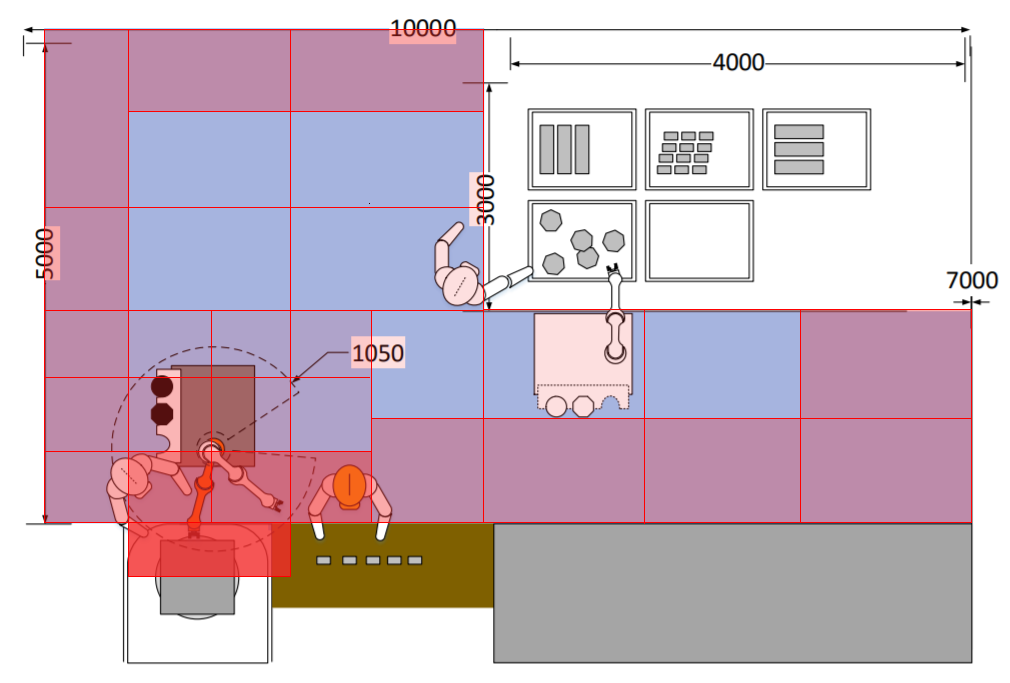
\includegraphics[width=\textwidth]{images/layout} 
\caption{Subdivision of the layout, highlighted areas are the most dangerous ones} 
\label{fig:layout} 
\end{figure}

\clearpage
The most critical areas are the ones with indices from 1 to 12, particular attention must be paid to L\textsubscript0 too, since it is where the EE and O could be working together. 

\begin{figure}[htp] 
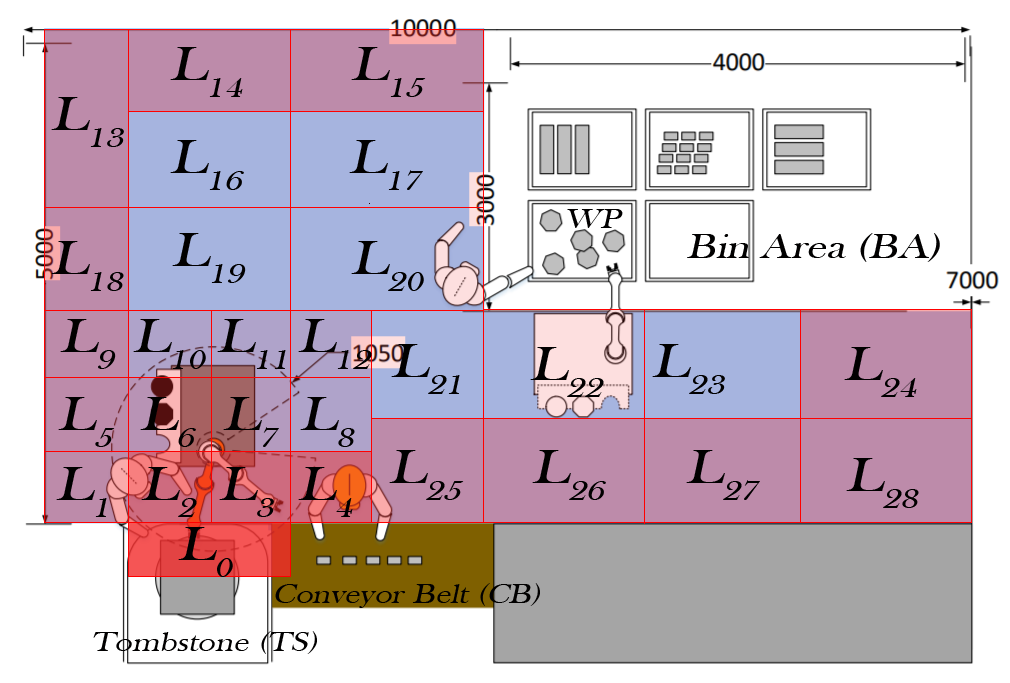
\includegraphics[width=\textwidth]{images/layoutnames} 
\caption{Names of the splitted layout and various areas} 
\label{fig:layout} 
\end{figure}

\begin{itemize}
	\item \textbf{..}:\@ ..
\end{itemize}

\subsection{Sensors? signals?}
\clearpage
\section{Archi-TRIO model}




\clearpage
\section{TRIO specification}
\begin{equation*}
\lasttime(F, t) = \past(F, t) \land \lasted(\lnot F, t)
\end{equation*}

\section{Model checking}

\pagebreak
\appendix
\section{Area modeling}

\begin{align*}
&\neg Adj(L0, L0) \land Adj(L0, L1) \land Adj(L0, L2) \land Adj(L0, L3) \land Adj(L0, L4) \land \neg Adj(L0, L5) \land \neg Adj(L0, L6) \\
&\land \neg Adj(L0, L7) \land \neg Adj(L0, L8) \land \neg Adj(L0, L9) \land \neg Adj(L0, L10) \land \neg Adj(L0, L11) \land \neg Adj(L0, L12) \\
&\land \neg Adj(L0, L13) \land \neg Adj(L0, L14) \land \neg Adj(L0, L15) \land \neg Adj(L0, L16) \land \neg Adj(L0, L17) \land \neg Adj(L0, L18) \\
&\land \neg Adj(L0, L19) \land \neg Adj(L0, L20) \land \neg Adj(L0, L21) \land \neg Adj(L0, L22) \land \neg Adj(L0, L23) \land \neg Adj(L0, L24) \\
&\land \neg Adj(L0, L25) \land \neg Adj(L0, L26) \land \neg Adj(L0, L27) \land \neg Adj(L0, L28) \land Adj(L1, L0) \land \neg Adj(L1, L1) \land Adj(L1, L2) \\
&\land \neg Adj(L1, L3) \land \neg Adj(L1, L4) \land Adj(L1, L5) \land Adj(L1, L6) \land \neg Adj(L1, L7) \land \neg Adj(L1, L8) \land \neg Adj(L1, L9) \\
&\land \neg Adj(L1, L10) \land \neg Adj(L1, L11) \land \neg Adj(L1, L12) \land \neg Adj(L1, L13) \land \neg Adj(L1, L14) \land \neg Adj(L1, L15) \\
&\land \neg Adj(L1, L16) \land \neg Adj(L1, L17) \land \neg Adj(L1, L18) \land \neg Adj(L1, L19) \land \neg Adj(L1, L20) \land \neg Adj(L1, L21) \\
&\land \neg Adj(L1, L22) \land \neg Adj(L1, L23) \land \neg Adj(L1, L24) \land \neg Adj(L1, L25) \land \neg Adj(L1, L26) \land \neg Adj(L1, L27) \\
&\land \neg Adj(L1, L28) \land Adj(L2, L0) \land Adj(L2, L1) \land \neg Adj(L2, L2) \land Adj(L2, L3) \land \neg Adj(L2, L4) \land Adj(L2, L5) \\
&\land Adj(L2, L6) \land Adj(L2, L7) \land \neg Adj(L2, L8) \land \neg Adj(L2, L9) \land \neg Adj(L2, L10) \land \neg Adj(L2, L11) \\
&\land \neg Adj(L2, L12) \land \neg Adj(L2, L13) \land \neg Adj(L2, L14) \land \neg Adj(L2, L15) \land \neg Adj(L2, L16) \land \neg Adj(L2, L17) \\
&\land \neg Adj(L2, L18) \land \neg Adj(L2, L19) \land \neg Adj(L2, L20) \land \neg Adj(L2, L21) \land \neg Adj(L2, L22) \land \neg Adj(L2, L23) \\
&\land \neg Adj(L2, L24) \land \neg Adj(L2, L25) \land \neg Adj(L2, L26) \land \neg Adj(L2, L27) \land \neg Adj(L2, L28) \land Adj(L3, L0) \\
&\land \neg Adj(L3, L1) \land Adj(L3, L2) \land \neg Adj(L3, L3) \land Adj(L3, L4) \land \neg Adj(L3, L5) \land Adj(L3, L6) \\
&\ldots 
\end{align*}
\end{document}